\documentclass{article}

\usepackage{assign}
\setcoursetitle{CS698X: Topics in Probabilistic Modelling and Inference}
\setassigncode{1}
\setstartnewpage{TRUE}

\begin{document}
\makeheader

Please note that I have attempted all the questions, with each subsequent question starting from a new page.

\begin{question}

	Below, I state the notations, terms given to us and some observations.

	\begin{enumerate}[label=\bt{\theenumi.}]
		\ditem[Likelihood]
			\begin{align*}
				\prob{\vy \pipe X, \vw, \beta}	\eq	\prod_{n = 1}^N \ND{y_n \pipe \tr{\vw} \vx_n, \beta^{-1}}
			\end{align*}
		\item Let $\vlambda$ represent $\tr{\brac{\lambda_1, \lambda_2 \dots \lambda_d}}$ and $\Lambda$ represent the $D \times D$ diagonal matrix with element at $(d, d)$ be equal to $\lambda_d$
		\ditem[Prior]
			\begin{align*}
				\prob{\vw \pipe \vlambda}	\eq	\prod_{d = 1}^D \ND{w_d \pipe 0, \lambda_d^{-1}}
			\end{align*}
	\end{enumerate}

	\begin{qpart}{A}

		I will show that in both the cases, the marginal has a closed form, however will be showing the working for only the second case \ie all $\lambda_d$'s are different, and then simplify for the first case by putting $\qforall d \in \brac{D}, \lambda_d = \lambda$.

		In order to compute the marginal likelihood, we can compute the posterior of our parameter \ie $\vw$, and then use Bayes Rule to compute the marginal likelihood.
		\begin{equation}
			\prob{\vy \pipe X, \beta, \vlambda}	\eq	\frac{\prob{\vy \pipe X, \vw, \beta} \prob{\vw \pipe \vlambda}}{\prob{\vw \pipe \vy, X, \beta, \vlambda}}
			\label{eq:q1-bayes}
		\end{equation}

		We start by computing the posterior over $\vw$.
		\begin{align*}
			\prob{\vw \pipe \vy, X, \beta, \vlambda}	&\qprop	\prob{\vy \pipe X, \vw, \beta} \prob{\vw \pipe \vlambda} \\
			&\qprop	\prod_{n = 1}^N \ND{\tr{\vw} \vx_n, \beta^{-1}} \prod_{d = 1}^D \ND{0, \lambda_d^{-1}} \\
			&\qprop \prod_{n = 1}^N \texp{\frac{-\beta}{2} \para{y_n - \tr{\vw} \vx_n}^2} \prod_{d = 1}^D \texp{\frac{-\lambda_d}{2} \para{w_d}^2} \\
			&\qprop \texp{\frac{-1}{2} \para{ \beta \sum_{n = 1}^N \para{y_n - \tr{\vw} \vx_n}^2 + \sum_{d = 1}^D \lambda_d w_d^2}} \\
			&\qprop	\texp{\frac{-1}{2} \para{\beta \tr{\vw} \tr{X} X \vw - 2 \tr{\vw} \tr{X} \vy + \tr{\vw} \Lambda \vw}}
		\end{align*}

		\note{I have ignored all terms independent of $\vw$ during the above computations}

		The last term looks like a Gaussian distribution, and hence, we can use the Completing the Squares trick to find out the exact distribution.
		Therefore, we get
		\begin{equation}
			\prob{\vw \pipe \vy, X, \beta, \vlambda}	\eq \ND{\vw \pipe \vmu_w, \Sigma_w}
			\label{eq:q1-posterior}
		\end{equation}

		where
		\begin{align*}
			\Sigma_w	&\eq	\para{\beta \tr{X} X + \Lambda}^{-1} \\
			\vmu_w		&\eq	\para{\tr{X} X + \frac{1}{\beta} \Lambda}^{-1} \tr{X} \vy
		\end{align*}

		Therefore, we have the posterior.
		Now we can put this in Equation \ref{eq:q1-bayes}.
		\begin{align*}
			\prob{\vy \pipe X, \beta, \vlambda}	&\eq	\frac{\prob{\vy \pipe X, \vw, \beta} \prob{\vw \pipe \vlambda}}{\prob{\vw \pipe \vy, X, \beta, \vlambda}} \\
			&\qprop	\texp{\frac{-1}{2} \para{\beta \sum_{n = 1}^N y_n^2 + \beta \tr{\vw} \tr{X} X \vw - 2 \beta \tr{\vw} \tr{X} \vy + \tr{\vw} \Lambda \vw} \\ &\quad\quad\quad+ \frac{1}{2} \para{\tr{\para{\vw - \vmu_w}} \Sigma_w^{-1} \para{\vw - \vmu}}} \\
			&\qprop	\texp{\frac{-1}{2} \para{\beta \sum_{n = 1}^N y_n^2 - \tr{\vmu_w} \Sigma_w^{-1} \vmu_w }}
		\end{align*}
		Putting $\vmu_w = \beta \cdot \Sigma_w \tr{X} \vy$,
		\begin{align*}
			\prob{\vy \pipe X, \beta, \vlambda}	&\qprop	\texp{\frac{-1}{2} \para{\beta \sum_{n = 1}^N y_n^2 - \tr{\para{\beta \cdot \Sigma_w \tr{X} \vy}} \Sigma_w^{-1} \beta \cdot \Sigma_w \tr{X} \vy}} \\
			&\qprop	\texp{\frac{-1}{2} \para{\tr{\vy} \para{\beta \vI - \beta^2 X \tr{\Sigma_w} \tr{X}} \vy}}
		\end{align*}

		This again is a gaussian distribution.
		Therefore, we can write the final form of this distribution as follows
		\begin{equation}
			\prob{\vy \pipe X, \beta, \vlambda}	\eq	\ND{\vy \pipe \vzero, \Sigma}
		\end{equation}
		where $\Sigma = \para{\beta\, \vI - \beta^2\, X\, \Sigma_w\, \tr{X}}^{-1}$

		We can further simplify the term of the gaussian using a property of matrix inverses.
		Consider the inverse property given in Equation 166 in \cite{matrix-cookbook}, which states
		\begin{equation}
			\para{\vI + AB}^{-1}	\eq	\vI - A \para{\vI + BA}^{-1} B
			\label{eq:q1-matrix-inverse}
		\end{equation}

		First let us rewrite $\Sigma$
		\begin{align*}
			\Sigma	&\eq	\frac{1}{\beta} \para{\vI - \beta X \para{\beta \tr{X} X + \Lambda}^{-1} \tr{X}} \\
			\implies \beta\ \Sigma	&\eq	\para{\vI + \para{- X \para{\tr{X} X + \frac{1}{\beta} \Lambda}^{-1}} \tr{X}}
		\end{align*}

		We want to represent this in the form of the term given in the LHS of Equation \ref{eq:q1-matrix-inverse}.

		Therefore, let $A = \para{- X \para{\tr{X} X + \frac{1}{\beta} \Lambda}^{-1}}$ and $B = \tr{X}$.
		Then

		\begin{align*}
			\beta\ \Sigma	&\eq	\para{\vI + AB}^{-1} \\
			&\eq	\vI - A \para{\vI + BA}^{-1} B \\
			&\eq	\vI - A \para{\vI - \tr{X} X \para{\tr{X} X + \frac{\Lambda}{\beta}}^{-1}}^{-1} B \\
			&\eq	\vI - A \para{\vI - \para{\tr{X} X + \frac{\Lambda}{\beta} - \frac{\Lambda}{\beta}} \para{\tr{X} X + \frac{\Lambda}{\beta}}^{-1}}^{-1} B \\
			&\eq	\vI - A \para{\frac{\Lambda}{\beta} \para{\tr{X} X + \frac{\Lambda}{\beta}}^{-1}}^{-1} B \\
			&\eq	\vI - \para{- X \para{\tr{X} X + \frac{\Lambda}{\beta}}^{-1} \para{\tr{X} X + \frac{\Lambda}{\beta}} \para{\frac{\Lambda}{\beta}}^{-1}} \tr{X} \\
			&\eq	\vI + \beta X \Lambda^{-1} \tr{X} \\
			\implies \Sigma	&\eq	\frac{1}{\beta} \vI + X \Lambda^{-1} \tr{X}
		\end{align*}

		Hence, we can now rewrite our answer,
		\answer[0.5\textwidth]{
			\begin{equation}
				\prob{\vy \pipe X, \beta, \vlambda}	\eq	\ND{\vy \pipe, \vzero, \Sigma}
				\label{eq:q1-marginal}
			\end{equation}
		}
		where $\Sigma = \beta^{-1} \vI + X \Lambda^{-1} \tr{X}$

		If for all $d = 1 \dots D$, $\lambda_d = \lambda$, we can simply put this in the result obtained in Equation \ref{eq:q1-marginal}

	\end{qpart}

	\begin{qpart}{B}

		As discussed in class, we do MLE-II inference by performing MLE on the marginal likelihood $\prob{\vy \pipe X, \beta, \vlambda}$, and then approximate the posterior using the conditional posterior of $\vw$ $\para{\prob{\vw \pipe \vy, X, \wbeta, \widehat{\vlambda}}}$.
		\br

		\note{We define $\vlambda$ and $\Lambda$ the same as in part A}

		Taking a cue from the MLE-II derivation given in PRML 3.5 \cite{prml}, we represent the marginal in a different manner, and then try to maximize it for the purpose of MLE.
		\begin{align*}
			\prob{\vy \pipe X, \beta, \vlambda}	&\eq	\int_{\vw} \prob{\vy \pipe X, \vw, \beta} \prob{\vw \pipe X, \beta, \vlambda} \id \vw \\
			&\eq	\para{\frac{\beta}{2\pi}}^{\frac{N}{2}} \sqrt{\frac{\abs{\Lambda}}{\para{2 \pi}^D}} \int_{\vw} \texp{- E(\vw)} \id \vw
		\end{align*}
		where $E : \vw \mapsto \bR$ is the evidence function \cite{prml} and is defined as
		\begin{align*}
			E(\vw)	\eq	\frac{\beta}{2} \tr{\para{\vy - X \vw}} \para{\vy - X \vw} + \frac{1}{2} \tr{\vw} \Lambda \vw
		\end{align*}

		We can also represent $E(\vw)$ using $\vmu_w$ which is the mean of the posterior as derived in part A.
		\begin{align*}
			2 E(\vw)	&\eq	\beta \tr{\para{\vy - X \vmu_w - X (\vw - \vmu_w)}} \para{\vy - X \vmu_w - X (\vw - \vmu_w)} + \tr{\vw} \Lambda \vw \\
			&\eq	\beta \tr{\para{\vy - X \vmu_w}} \para{\vy - X \vmu_w}  + \tr{\para{\vw - \vmu_w}} \beta \tr{X} X \para{\vw - \vmu_w} - 2 \tr{\para{w - \vmu_w}} \beta \tr{X} \para{y - X \vmu_w}
		\end{align*}

		We can write $\beta \tr{X} \para{y - X \vmu_w}$ as $\Lambda \vmu_w$ by expanding $\vmu_w$ as shown below.
		\begin{align*}
			\vmu_w	&\eq	\beta \para{\beta \tr{X} X + \Lambda}^{-1} \tr{X} \vy \\
			\implies \beta \tr{X} \para{\vy - X \vmu_w}	&\eq	\beta \para{\vI - \beta \tr{X} X \para{\beta \tr{X} X + \Lambda}^{-1}} \tr{X} \vy \\
			&\eq	\beta \Lambda \para{\beta \tr{X} X + \Lambda}^{-1} \tr{X} \vy \\
			&\eq	\Lambda \vmu_w
		\end{align*}
		Therefore
		\begin{align*}
			E(\vw)	&\eq	\beta \tr{\para{\vy - X \vmu_w}} \para{\vy - X \vmu_w}  + \tr{\para{\vw - \vmu_w}} \beta \tr{X} X \para{\vw - \vmu_w} - 2 \tr{\para{w - \vmu_w}} \Lambda \vmu_w + \tr{\vw} \Lambda \vw \\
			&\eq	\beta \tr{\para{\vy - X \vmu_w}} \para{\vy - X \vmu_w} + \tr{\para{\vw - \vmu_w}} \beta \tr{X} X \para{\vw - \vmu_w} - 2 \tr{\vw} \Lambda \vmu_w + 2 \tr{\vmu_w} \Lambda \vmu_w + \tr{\vw} \Lambda \vw \\
			&\eq	\beta \tr{\para{\vy - X \vmu_w}} \para{\vy - X \vmu_w} + \tr{\para{\vw - \vmu_w}} \para{\beta \tr{X} X + \Lambda} \para{\vw - \vmu_w} + \tr{\vmu_w} \Lambda \vmu_w \\
			&\eq	2 E(\vmu_w) + \tr{\para{\vw - \vmu_w}} \Sigma^{-1} \para{\vw - \vmu_w}
		\end{align*}

		Hence, we can write
		\begin{equation}
			E(\vw)	\eq	E(\vmu_w) + \frac{1}{2} \tr{\para{\vw - \vmu_w}} \Sigma^{-1} \para{\vw - \vmu_w}
			\label{eq:q1-evidence-mean}
		\end{equation}

		We can now write the Marginal Likelihood in this form
		\begin{align*}
			\int_{\vw} \texp{- E(w)}	\eq	 \texp{- E(\vmu_w)} \int_{\vw} \texp{- \frac{1}{2} \tr{\para{\vw - \vmu_w}} \Sigma^{-1} \para{\vw - \vmu_w}}
		\end{align*}
		Since the integral is just over the exponent part of the posterior distribution of $\vw$, we can write
		\begin{align*}
			\int_{\vw} \texp{- E(w)}	\eq	\texp{- E(\vmu_w)} \sqrt{\para{2 \pi}^D \abs{\Sigma}}
		\end{align*}

		Hence, the negative log marginal (NLM) can be written as
		\begin{equation}
			- \log{\prob{\vy \pipe X, \beta, \vlambda}}	\eq	E(\vmu_w) + \frac{1}{2} \log{\abs{\Sigma_w^{-1}}} - \frac{1}{2} \log{\abs{\Lambda}} - \frac{N}{2} \log{\beta} + \mt{constants}
			\label{eq:q1-marginal-alt}
		\end{equation}

		Now, we can use iterative MLE-II scheme to solve for the hyperparamters.

		Suppose we have estimates of $\beta$ and $\vlambda$ as $\beta^t$ and $\vlambda^t$ from the t\tth iteration of the MLE-II scheme, then we can compute the conditional posterior of $\vw$ given these estimates.
		Note, we have already computed this posterior, as given in Equation \ref{eq:q1-posterior}.
		Therefore, we can write
		\begin{align*}
			\prob{\vw^{t + 1} \pipe \vy, X, \beta^t, \vlambda^t}	\eq	\ND{\vw^{t + 1} \pipe \vmu_w^t, \Sigma_w^t}
		\end{align*}
		where
		\begin{align*}
			\Sigma_w^t	&\eq	\para{\beta^t \tr{X} X + \Lambda^t}^{-1} \\
			\vmu_w^t	&\eq	\para{\tr{X} X + \frac{1}{\beta^t} \Lambda^t}^{-1} \tr{X} \vy
		\end{align*}

		Now, we can continue with the point estimation step of the MLE-II method, \ie estimating the update values $\beta^{t + 1}$ and $\vlambda^{t + 1}$.
		\begin{align*}
			\beta^{t + 1}, \vlambda^{t + 1}	\eq	\argmin{\beta, \vlambda} - \log{\prob{\vy \pipe X, \beta, \vlambda}}
		\end{align*}

		Since we wish to minimize the NLM (negative log marginal) given in the above equation, we can equate the partial derivatives of $\beta$ and $\vlambda$ at $\beta = \beta^{t + 1}$ and $\qforall d \in \brac{D} \lambda_d = \vlambda_d^{t + 1}$ to 0.
		First, solving for $\lambda_d^{t + 1}$,
		\begin{align*}
			\brac{\derp{\text{NLM}}{\lambda_d}}_{\lambda_d = \lambda_d^{t + 1}}	\eq	0
		\end{align*}
		Usign Equations 36, 42, 49 and 70 from the Matrix Cookbook \cite{matrix-cookbook}, and replacing the NLM with the derived term in equation \ref{eq:q1-marginal-alt}
		\begin{align*}
			0	&\eq	\brac{\frac{1}{2} \derp{\tr{\vmu_w} \Lambda \vmu_w}{\lambda_d} +  \frac{1}{2} \trace{\Sigma_w \derp{\Sigma_w^{-1}}{\lambda_d}} - \frac{1}{2 \lambda_d}}_{\lambda_d = \lambda_d^{t + 1}} \\
		\end{align*}

		Using Jacobi's method for solving non-linear equations, let us say that we know the value of $\vmu_w$ \ie we estimate $\vmu_w = \vmu_w^t$ and $\Sigma = \Sigma^t$, therefore, we can write
		\begin{align*}
			\brac{\frac{1}{2} \mu_{w, d}^2 +  \frac{1}{2} \trace{\Sigma_w \derp{\beta \tr{X} X + \Lambda}{\lambda_d}} - \frac{1}{2 \lambda_d}}_{\lambda_d = \lambda_d^{t + 1}}	&\eq	0 \\
			\implies \set{\lambda_d^{t + 1}}^{-1}	&\eq	\set{\mu_{w, d}^t}^2 + \set{\Sigma_w^t}_{(d, d)}
		\end{align*}

		If for all $d \in \brac{D}$, $\lambda_d = \lambda$, we cannot write the above, since the derivatives in that case would be different.
		In that case, we follow the same procedure, but will obtain the following update equation
		\begin{align*}
			\set{\lambda^{t + 1}}^{-1}	\eq	\frac{1}{D} \brac{\tr{\set{\vmu_w^t}} \set{\vmu_w^t} + \trace{\Sigma_w^t}}
		\end{align*}

		Now, we can also give an update equation for $\beta$, following the same steps.
		\begin{align*}
			0	&\eq	\brac{\derp{NLM}{\beta}}_{\beta = \beta^{t + 1}} \\
			&\eq	\brac{\frac{1}{2} \tr{\para{\vy - X \vmu_w^t}} \para{\vy - X \vmu_w^t} + \frac{1}{2} \trace{\Sigma_w^t \tr{X} X} - \frac{N}{2 \beta}}_{\beta = \beta^{t + 1}} \\
			\implies \set{\beta^{t + 1}}^{-1}	&\eq	\frac{1}{N} \brac{\tr{\para{\vy - X \vmu_w^t}} \para{\vy - X \vmu_w^t} + \trace{\Sigma_w^t \tr{X} X}}
		\end{align*}

		Since this is independent of the $\Lambda$, we can say that for both the cases, the updation of $\beta$ will be the same.

		Therefore, we give an iterative algorithm for this (as discussed in class) in \hyperlink{algo:1}{Algorithm 1}

		\begin{algo}[0.9\textwidth]{h!}{MLE-II for Hyperparameter Estimation}

			\begin{enumerate}
				\item Assume some initial estimates for the hyperparamters, $\beta^0$ and $\vlambda^0$
				\item Repeat until convergence for t = $0, 1 \dots$
					\begin{enumerate}
						\item Estimate the posterior over $\vw^{t + 1}$ as
							\begin{align*}
								\prob{\vw^{t + 1} \pipe \vy, X, \vbeta^t, \vlambda^t}	\eq	\ND{\vw^{t + 1} \pipe \vmu_w^t, \Sigma_w^t}
							\end{align*}
							where
							\begin{align*}
								\Sigma_w^t	&\eq	\para{\beta^t \tr{X} X + \Lambda^t}^{-1} \\
								\vmu_w^t	&\eq	\beta^t \Sigma^t \tr{X} \vy
							\end{align*}
						\item Re-esimate the hyperparameters as

							\begin{align*}
								\set{\beta^{t + 1}}^{-1}	&\eq	\frac{1}{N} \brac{\tr{\para{\vy - X \vmu_w^t}} \para{\vy - X \vmu_w^t} + \trace{\Sigma_w^t \tr{X} X}}
							\end{align*}
							\bt{Case 1}
							\begin{align*}
								\forall\ d \in \brac{D},\ \set{\lambda_d^{t + 1}}^{-1}	&\eq	\set{\mu_{w, d}^t}^2 + \set{\Sigma_w^t}_{(d, d)}
							\end{align*}
							\bt{Case 2}
							\begin{align*}
								\set{\lambda^{t + 1}}^{-1}	\eq	\frac{1}{D} \brac{\tr{\set{\vmu_w^t}} \set{\vmu_w^t} + \trace{\Sigma_w^t}}
							\end{align*}
					\end{enumerate}
			\end{enumerate}

		\end{algo}

	\end{qpart}

\end{question}

\begin{question}

	We have the likelihood and the prior, and we want to find out the marginal likelihood.
	Given
	\begin{align*}
		\prob{x \pipe \lambda}				&\eq	\exp{-\lambda} \frac{\lambda^x}{\fact{x}} \\
		\prob{\lambda \pipe \alpha, \beta}	&\eq	\frac{\beta^\alpha}{\Gamma(\alpha)} \lambda^{\alpha - 1} \exp{- \beta \lambda}
	\end{align*}

	Therefore, the marginal likelihood can be written as
	\begin{align*}
		\prob{x \pipe \alpha, \beta}		&\eq	\int_{\lambda} \exp{-\lambda} \frac{\lambda^x}{\fact{x}} \cdot \frac{\beta^\alpha}{\Gamma(\alpha)} \lambda^{\alpha - 1} \exp{- \beta \lambda} \\
		&\eq	\frac{\beta^\alpha}{\fact{x} \, \Gamma(\alpha)} \int_{\lambda} \lambda^{x + \alpha - 1} \exp{-(1 + \beta) \lambda} \;\text{d}\lambda
	\end{align*}

	Since the term inside the integral is a form of the gamma distribution, we can try to normalize it.
	\begin{align*}
		\prob{x \pipe \alpha, \beta}	&\eq	\frac{\beta^\alpha \, \Gamma(\alpha + x)}{\fact{x} \, \Gamma(\alpha) \, (1 + \beta)^{\alpha + x}} \int_{\lambda} \frac{(1 + \beta)^{\alpha + x}}{\Gamma(\alpha + x)} \lambda^{x + \alpha - 1} \exp{-(1 + \beta) \lambda} \;\text{d}\lambda
	\end{align*}

	As we know, the integral of a probability distribution is always 1, hence we can write
	\begin{align*}
		\prob{x \pipe \alpha, \beta}	&\eq	\frac{\beta^{\alpha} \, \Gamma(\alpha + x)}{\fact{x} \, \Gamma(\alpha) \, (1 + \beta)^{\alpha + x}}
	\end{align*}

	Putting in $\alpha = r$ and $\beta = \frac{1 - p}{p}$, we get
	\answer{
		\begin{align*}
			\prob{x \pipe r, p}	\eq	\frac{\Gamma(r + x) \, p^x (1 - p)^r}{\Gamma(r) \, \fact{x}}
		\end{align*}
	}

	Given $r \in \bN$, the above distribution would be \et{Negative Binomial Distribution}.

\end{question}

\begin{question}

	We have the likelihood and the the prior.
	\begin{align*}
		\mdef{Likelihood}	\prob{x \pipe \sigma^2}	&\eq	\ND{x \pipe 0, \sigma^2} & \\
		\mdef{Prior}	\prob{\sigma^2 \pipe \gamma}	&\eq	\texp{\sigma^2 \pipe \gamma^2 / 2} &
	\end{align*}

	We need to compute the marginal likelihood \ie $\prob{x \pipe \gamma}$.
	\begin{align*}
		\prob{x \pipe \gamma}	&\eq	\int_{\sigma^2} \prob{x \pipe \sigma^2} \prob{\sigma^2 \pipe \gamma} \; \text{d}\sigma^2 \\
		&\eq	\frac{\gamma^2}{2 \sqrt{2 \pi}} \int_{\sigma^2} \frac{1}{\sigma} \texp{- \frac{x^2}{2 \sigma^2}} \texp{- \frac{\gamma^2 \sigma^2}{2}} \; \text{d}\sigma^2
	\end{align*}

	As hinted in the assignment, let us consider the MGF of the probability distribution $\prob{x \pipe \gamma}$,
	\begin{align*}
		\E[x \,|\, \gamma]{\exp{sx}}	&\eq	\int_{x} \exp{sx}\, \prob{x \pipe \gamma} \id x \\
		&\eq	\int_{x} \exp{sx} \brac{\int_{\sigma^2} \frac{1}{\sigma} \texp{- \frac{x^2}{2 \sigma^2}} \texp{- \frac{\gamma^2 \sigma^2}{2}} \; \text{d}\sigma^2} \id x
	\end{align*}

	Since we can change the order of the integrals \cite{wiki-order-of-integration}, we will try to integrate $x$ first
	\begin{align*}
		\E[x \,|\, \gamma]{\exp{sx}}	&\eq \frac{\gamma^2}{2 \sqrt{2 \pi}} \int_{\sigma^2} \int_{x} \exp{sx} \frac{1}{\sigma} \texp{- \frac{x}{2 \sigma^2}} \texp{- \frac{\gamma^2 \sigma^2}{2}} \id x \cdot \id \sigma^2 \\
		&\eq	\frac{\gamma^2}{2 \sqrt{2 \pi}} \int_{\sigma^2} \frac{1}{\sigma} \texp{- \frac{\gamma^2 \sigma^2}{2}} \int_{x} \texp{- \frac{1}{2 \sigma^2} \para{x^2 - 2sx \sigma^2}} \id x \cdot \id \sigma^2
	\end{align*}

	We can manipulate the exponent part in the inner integral to represent a gaussian.
	Therefore
	\begin{align*}
		\E[x \,|\, \gamma]{\exp{sx}}	&\eq	\frac{\gamma^2}{2} \int_{\sigma^2} \texp{- \frac{\gamma^2 \sigma^2}{2} + \frac{s^2 \sigma^2}{2}} \int_{x} \frac{1}{\sqrt{2 \pi \sigma^2}} \texp{- \frac{1}{2 \sigma^2} \para{x^2 - 2sx \sigma^2 + s^2 \sigma^4}} \id x \cdot \id \sigma^2 \\
		&\eq	\frac{\gamma^2}{2} \int_{\sigma^2} \texp{- \frac{\gamma^2 \sigma^2}{2} + \frac{s^2 \sigma^2}{2}} \int_{x} \frac{1}{\sqrt{2 \pi \sigma^2}} \texp{- \frac{1}{2 \sigma^2} \para{x - s \sigma^2}^2} \id x \cdot \id \sigma^2\
	\end{align*}

	Since we are integrating a gaussian distribution over x, we will get 1 as the answer of the inner integration, hence, we can write
	\begin{align*}
		\E[x \,|\, \gamma]{\exp{sx}}	&\eq	\frac{\gamma^2}{2} \int_{\sigma^2} \texp{\frac{\sigma^2}{2} \para{s^2 - \gamma^2}} \id \sigma^2 \\
		&\eq	\frac{\gamma^2}{2} \frac{2}{s^2 - \gamma^2} \brac{\texp{\frac{\sigma^2}{2} \para{s^2 - \gamma^2}}}_0^\infty
	\end{align*}

	Clearly this will exist if and only if $s^2 \le \gamma^2$.
	Suppose this is true, \ie $\abs{s} \le \abs{\gamma}$, then
	\begin{align*}
		\text{MGF}	\eq	\E[x \,|\, \gamma]{\exp{sx}}	\eq	\frac{1}{1 - \frac{s^2}{\gamma^2}}
	\end{align*}

	Comparing with the various MGF in the list from \cite{wiki-mgf}, we can say that this is the MGF of a Laplace Distribution where $\mu = 0$ and $b = 1 / \gamma$.
	Therefore
	\answer[0.5\textwidth]{
		\begin{align*}
			x \pipe y	\qsim	\tfunc{Laplace}{0, \gamma^{-1}}
		\end{align*}
	}

	The plots of both the distributions $\prob{x \pipe \sigma^2}$ and $\prob{x \pipe \gamma}$ is given in Figure \ref{fig:q3-plot}

	\begin{figure}[h!]
		\centering
		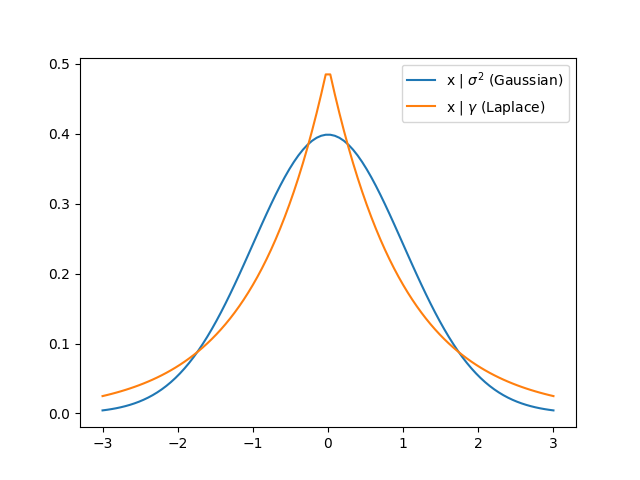
\includegraphics{includes/plots/q3/q3-plot.png}
		\caption{Comparasion of the Gaussian and Laplacian distributions for Question 3}
		\label{fig:q3-plot}
	\end{figure}

\end{question}

\begin{question}

	\begin{qsection}{Means and Covariances Observed}

		\begin{enumerate}
			\ditem[N = 1]
				\begin{align*}
					\mu_w		&\eq	\brac{
						\begin{matrix}
							-0.429 \\
							0.0226
						\end{matrix}
					} &
					\Sigma_w	&\eq	\brac{
						\begin{matrix}
							0.0382 &	0.0243	\\
							0.0243 &	0.4987	\\
						\end{matrix}
					}
				\end{align*}
			\ditem[N = 2]
				\begin{align*}
					\mu_w		&\eq	\brac{
						\begin{matrix}
							-0.336 \\
							0.6969
						\end{matrix}
					} &
					\Sigma_w	&\eq	\brac{
						\begin{matrix}
							0.0305 &	-0.032	\\
							-0.032 &	0.0899	\\
						\end{matrix}
					}
				\end{align*}
			\ditem[N = 5]
				\begin{align*}
					\mu_w		&\eq	\brac{
						\begin{matrix}
							-0.403 \\
							0.6885
						\end{matrix}
					} &
					\Sigma_w	&\eq	\brac{
						\begin{matrix}
							0.0239 &	-0.027	\\
							-0.027 &	0.0459	\\
						\end{matrix}
					}
				\end{align*}
			\ditem[N = 10]
				\begin{align*}
					\mu_w		&\eq	\brac{
						\begin{matrix}
							-0.275 \\
							0.4244
						\end{matrix}
					} &
					\Sigma_w	&\eq	\brac{
						\begin{matrix}
							0.0043 &	-0.002	\\
							0-.002 &	0.0102	\\
						\end{matrix}
					}
				\end{align*}
			\ditem[N = 20]
				\begin{align*}
					\mu_w		&\eq	\brac{
						\begin{matrix}
							-0.239 \\
							0.3688
						\end{matrix}
					} &
					\Sigma_w	&\eq	\brac{
						\begin{matrix}
							0.0020 &	-0.000	\\
							-0.000 &	0.0054	\\
						\end{matrix}
					}
				\end{align*}
		\end{enumerate}

	\end{qsection}

	\begin{qsection}{Plots for Values of $\vw$ Sampled from Posterior}

		The plots are shown in Figures 2 to 6

		\begin{figure}[h!]
			\centering
			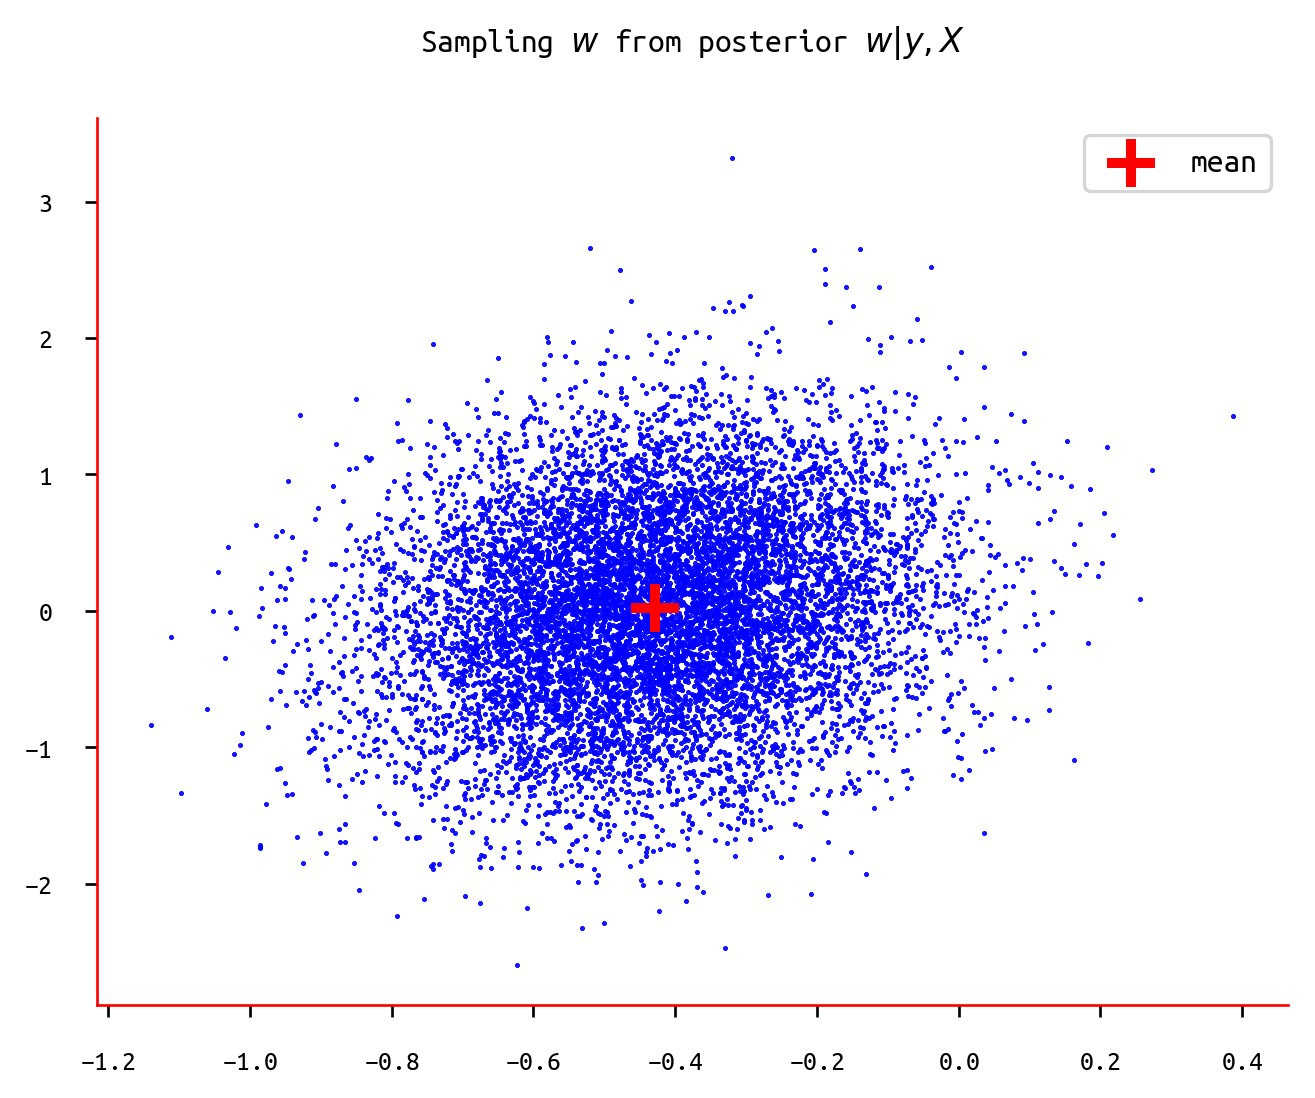
\includegraphics[height=275px]{includes/plots/q4b/posterior-samples-1.png}
			\caption{Sampling of $w$ for N = $1$}
		\end{figure}

		\begin{figure}[h!]
			\centering
			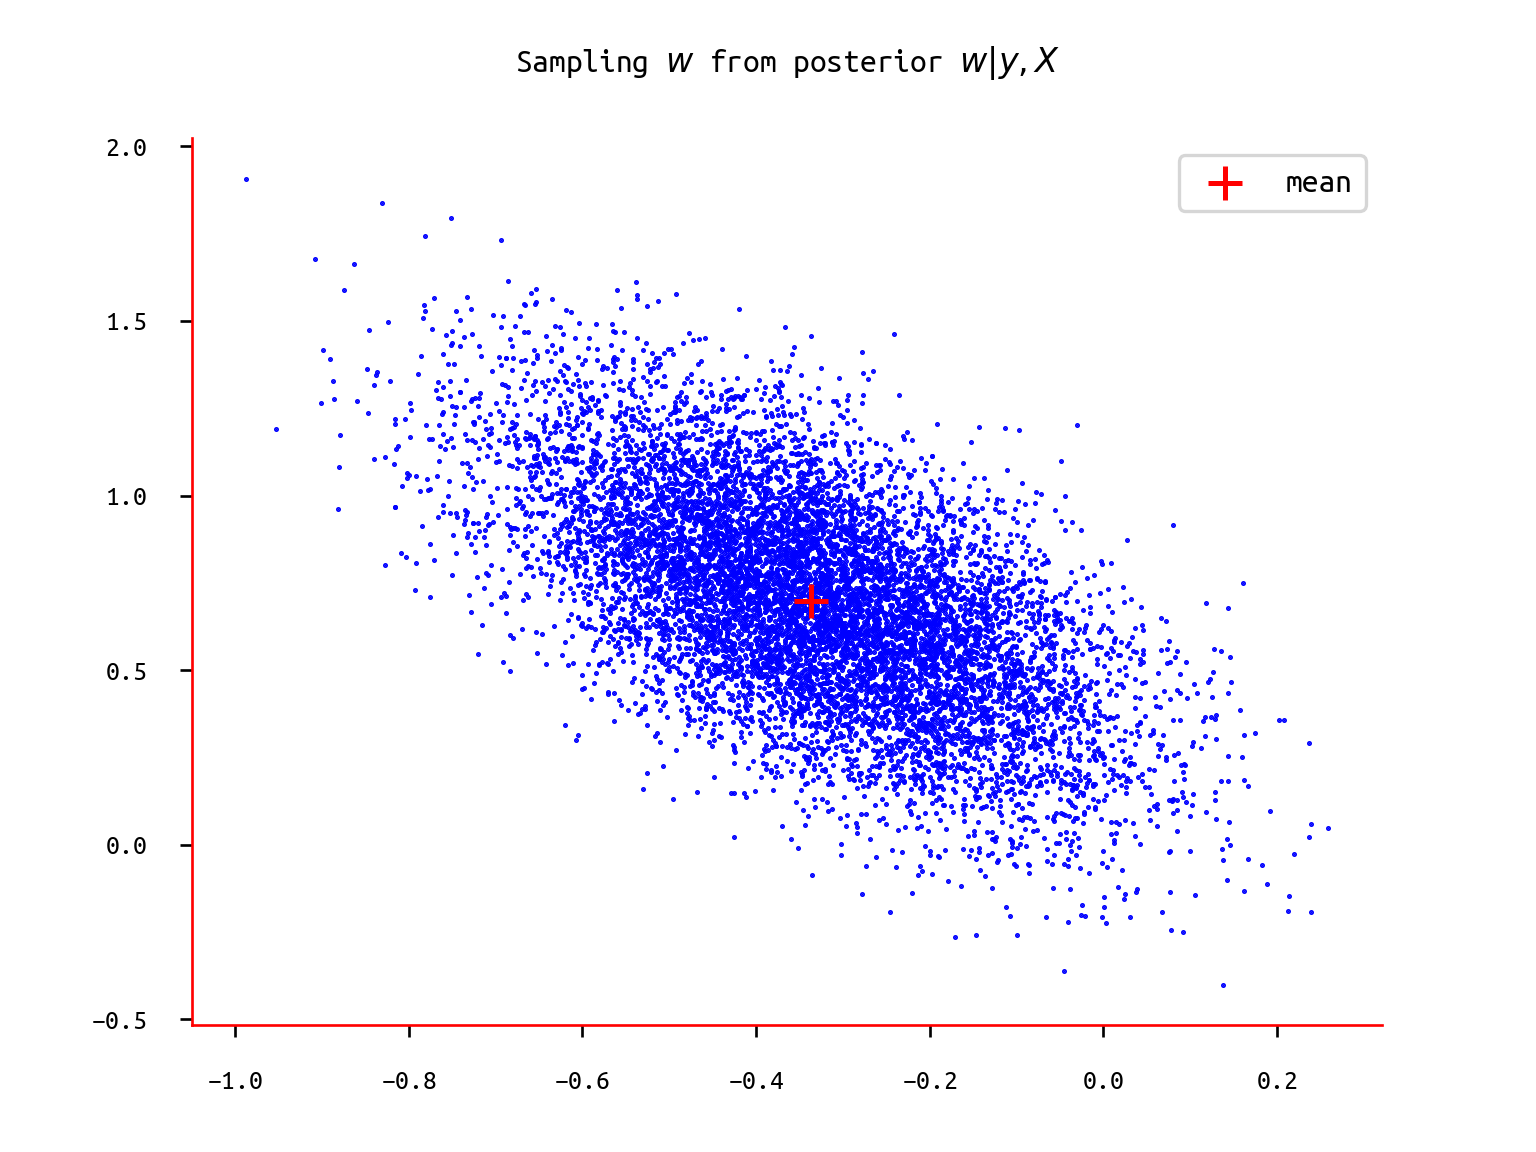
\includegraphics[height=275px]{includes/plots/q4b/posterior-samples-2.png}
			\caption{Sampling of $w$ for N = $2$}
		\end{figure}

		\begin{figure}[h!]
			\centering
			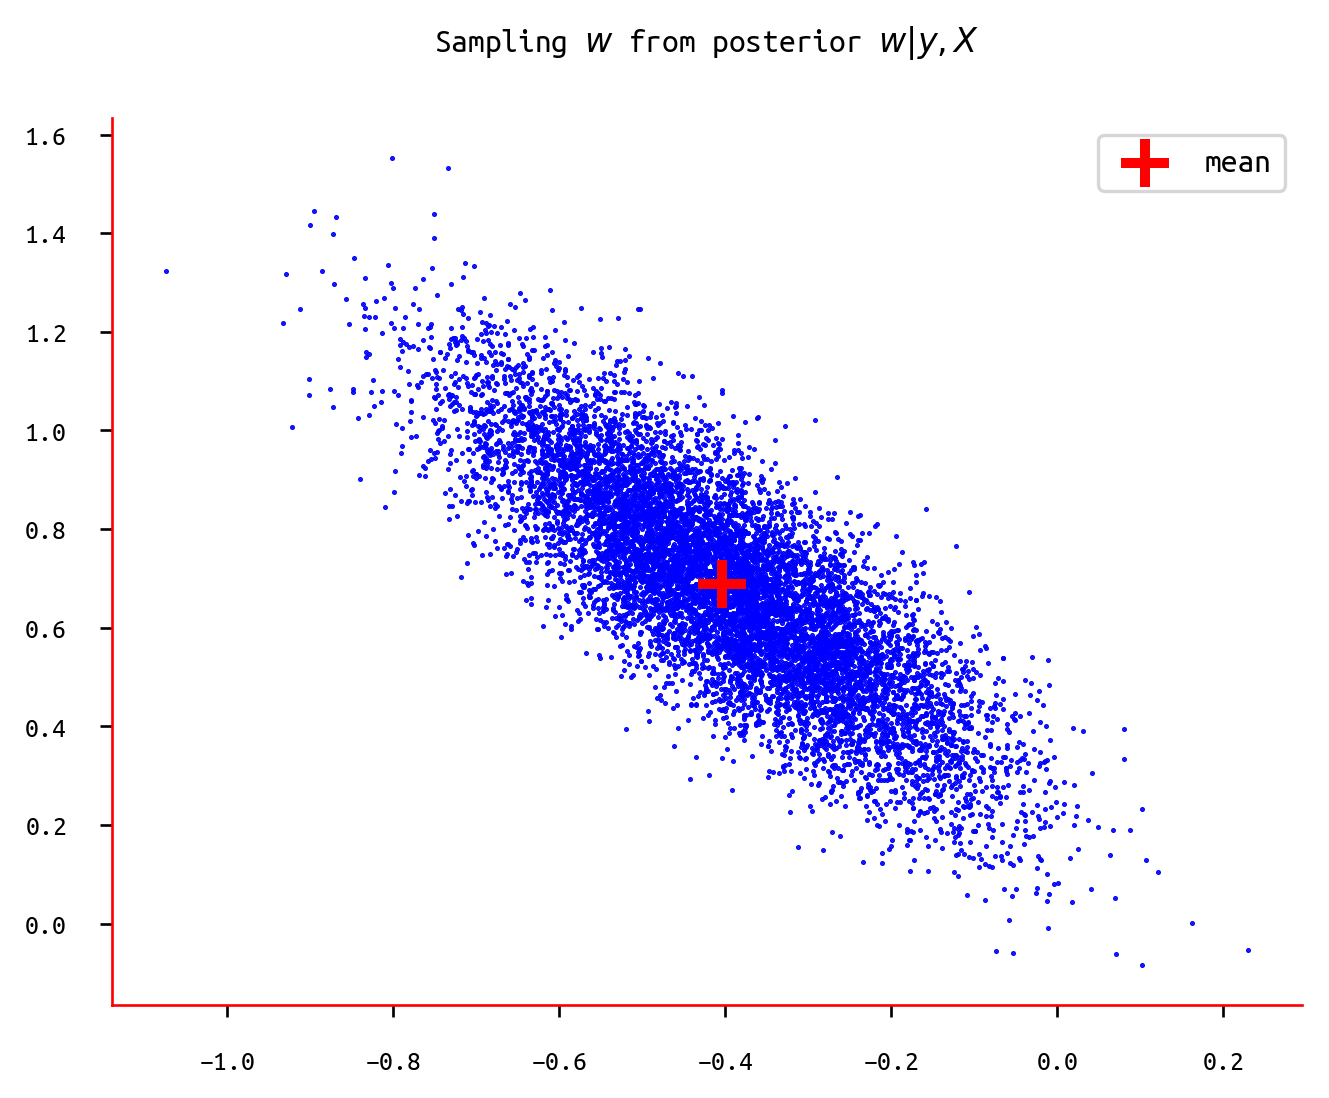
\includegraphics[height=275px]{includes/plots/q4b/posterior-samples-3.png}
			\caption{Sampling of $w$ for N = $5$}
		\end{figure}

		\begin{figure}[h!]
			\centering
			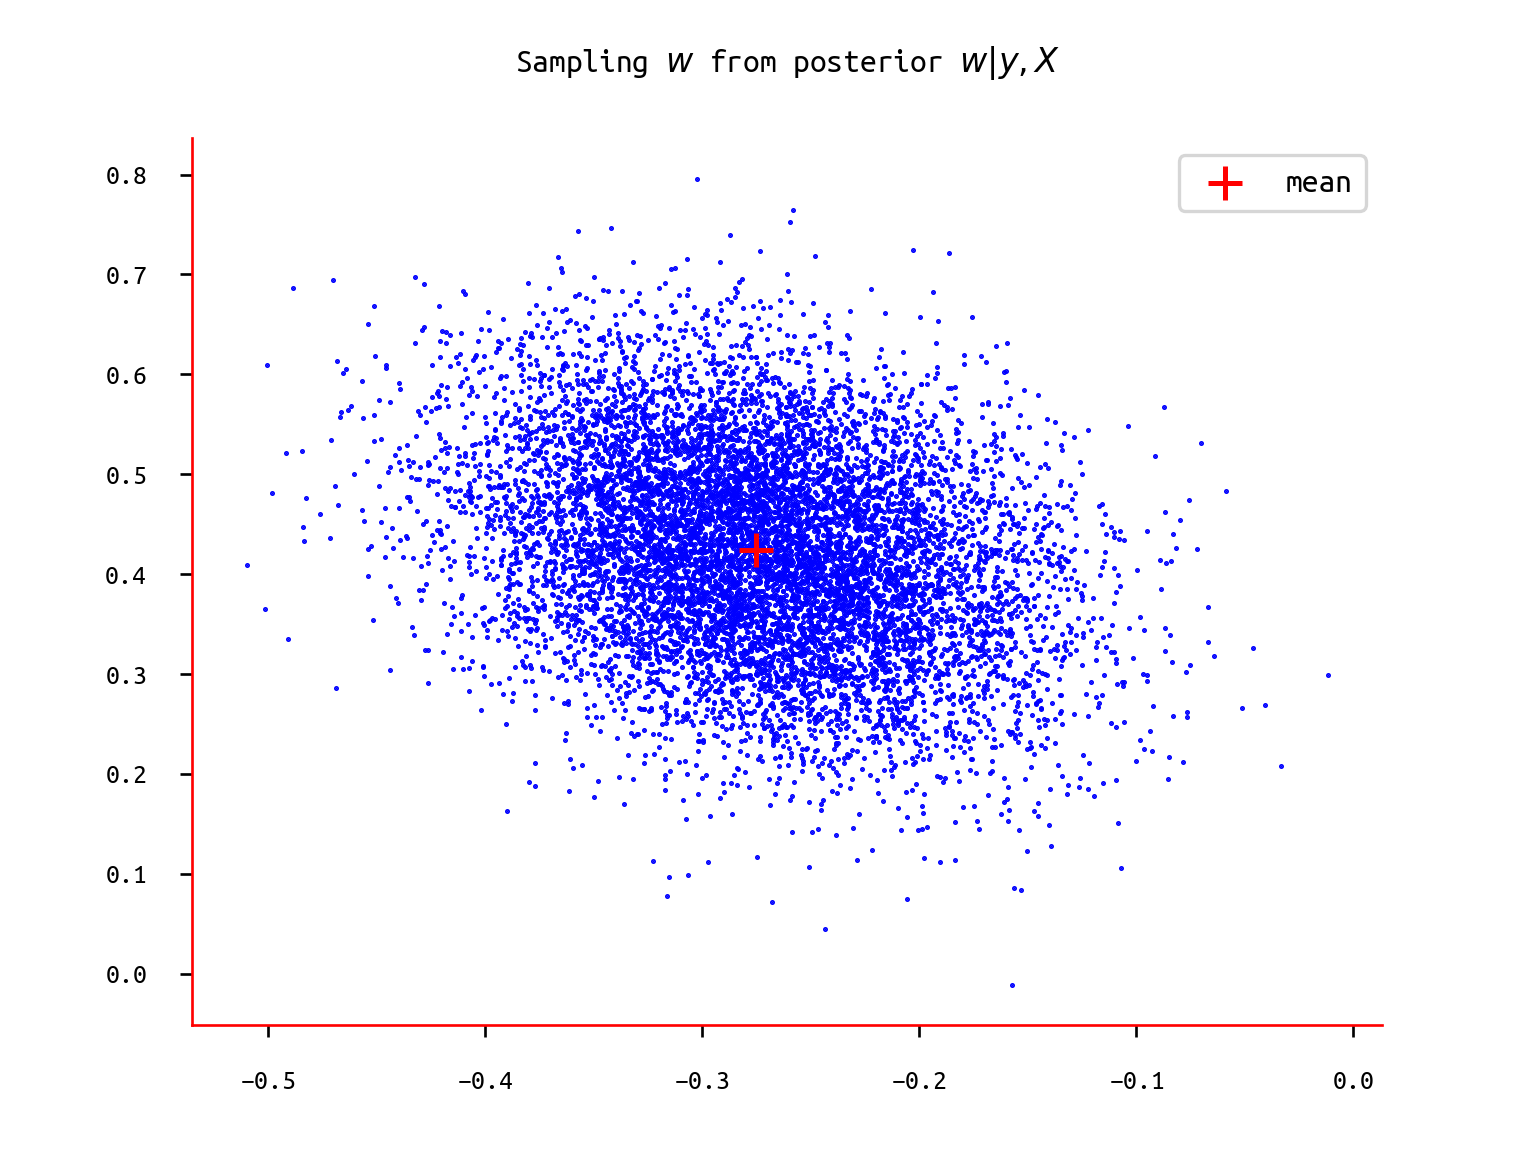
\includegraphics[height=275px]{includes/plots/q4b/posterior-samples-4.png}
			\caption{Sampling of $w$ for N = $10$}
		\end{figure}

		\begin{figure}[h!]
			\centering
			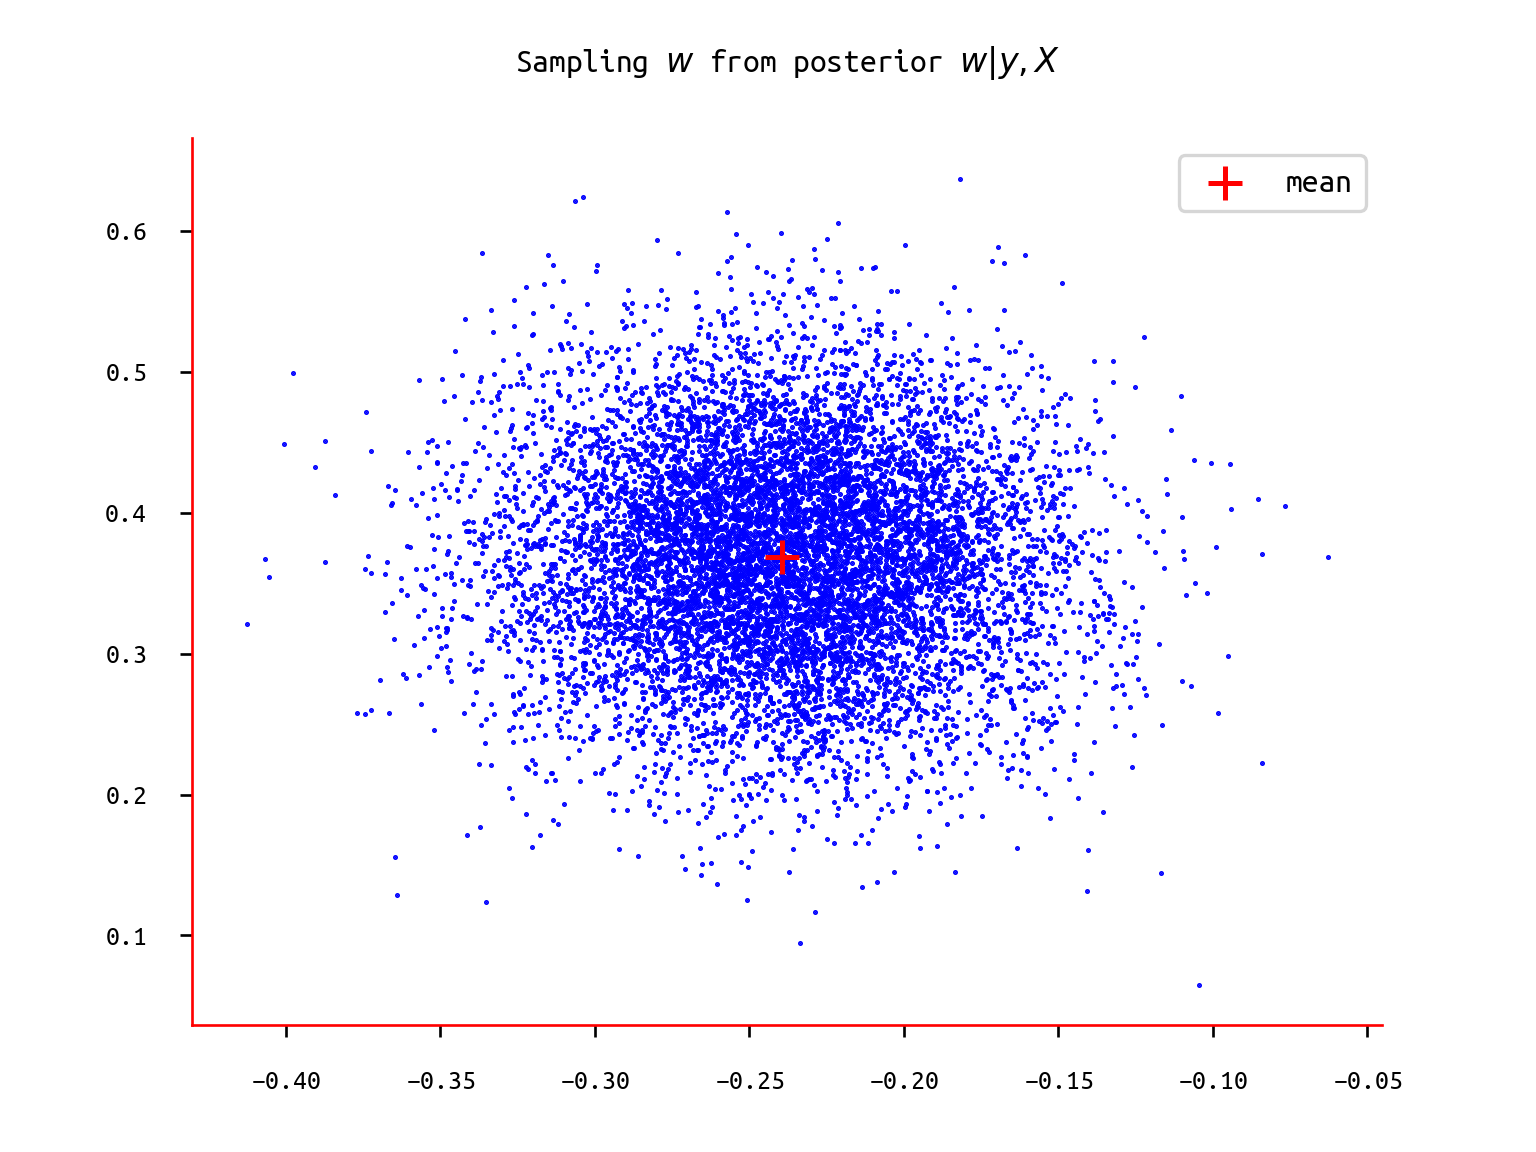
\includegraphics[height=275px]{includes/plots/q4b/posterior-samples-5.png}
			\caption{Sampling of $w$ for N = $20$}
		\end{figure}

	\end{qsection}

	\begin{qsection}{Plots for Prediction Lines for Sampled Values of $\vw$}

		The plots are shown in Figures 7 to 11

		\begin{figure}[h!]
			\centering
			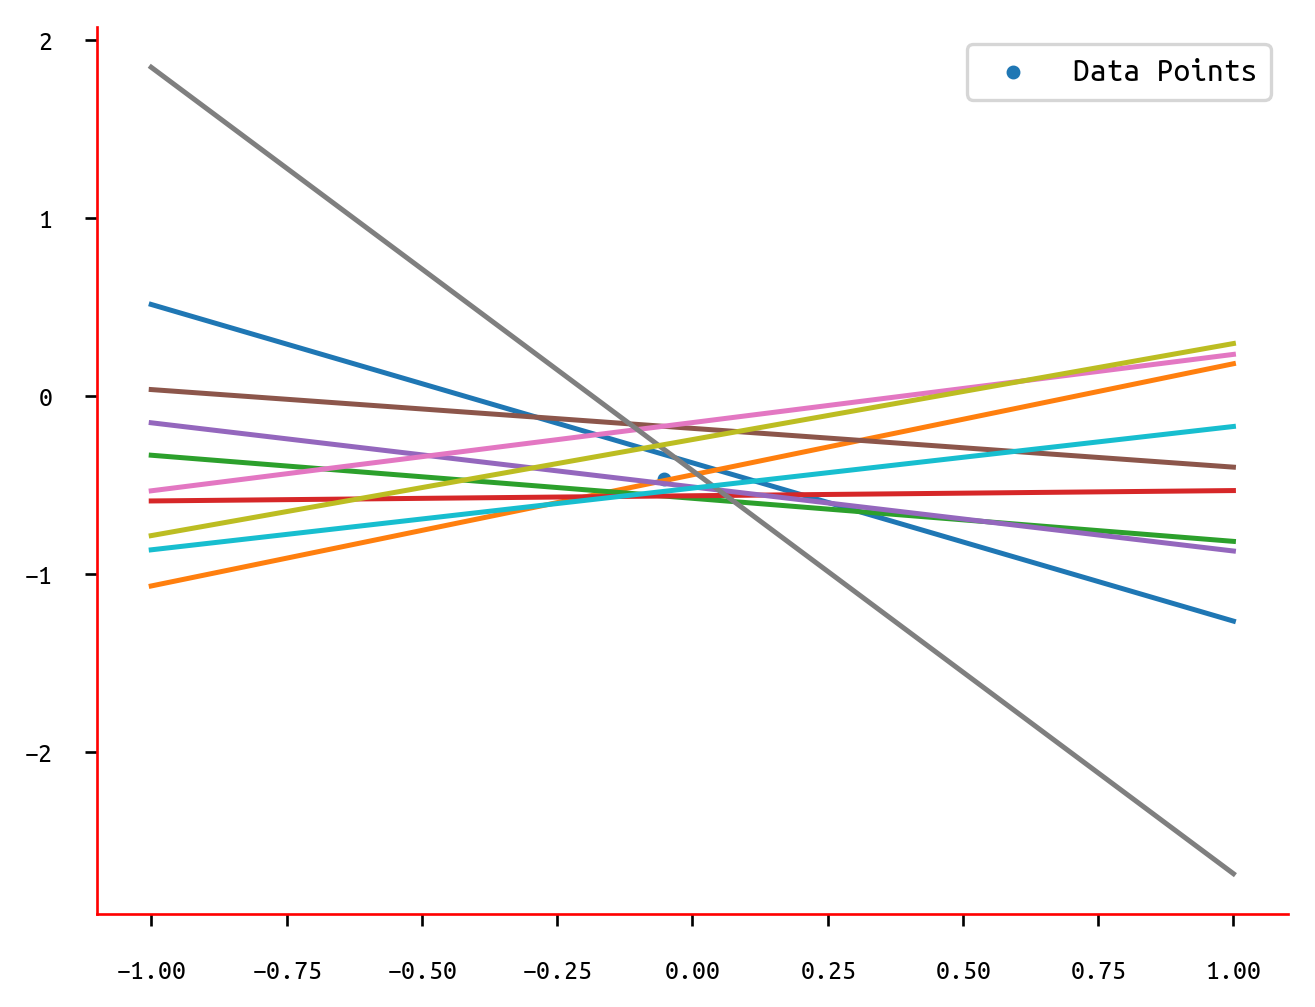
\includegraphics[height=275px]{includes/plots/q4c/predictive-models-1.png}
			\caption{Sampling of $w$ for N = $1$}
		\end{figure}

		\begin{figure}[h!]
			\centering
			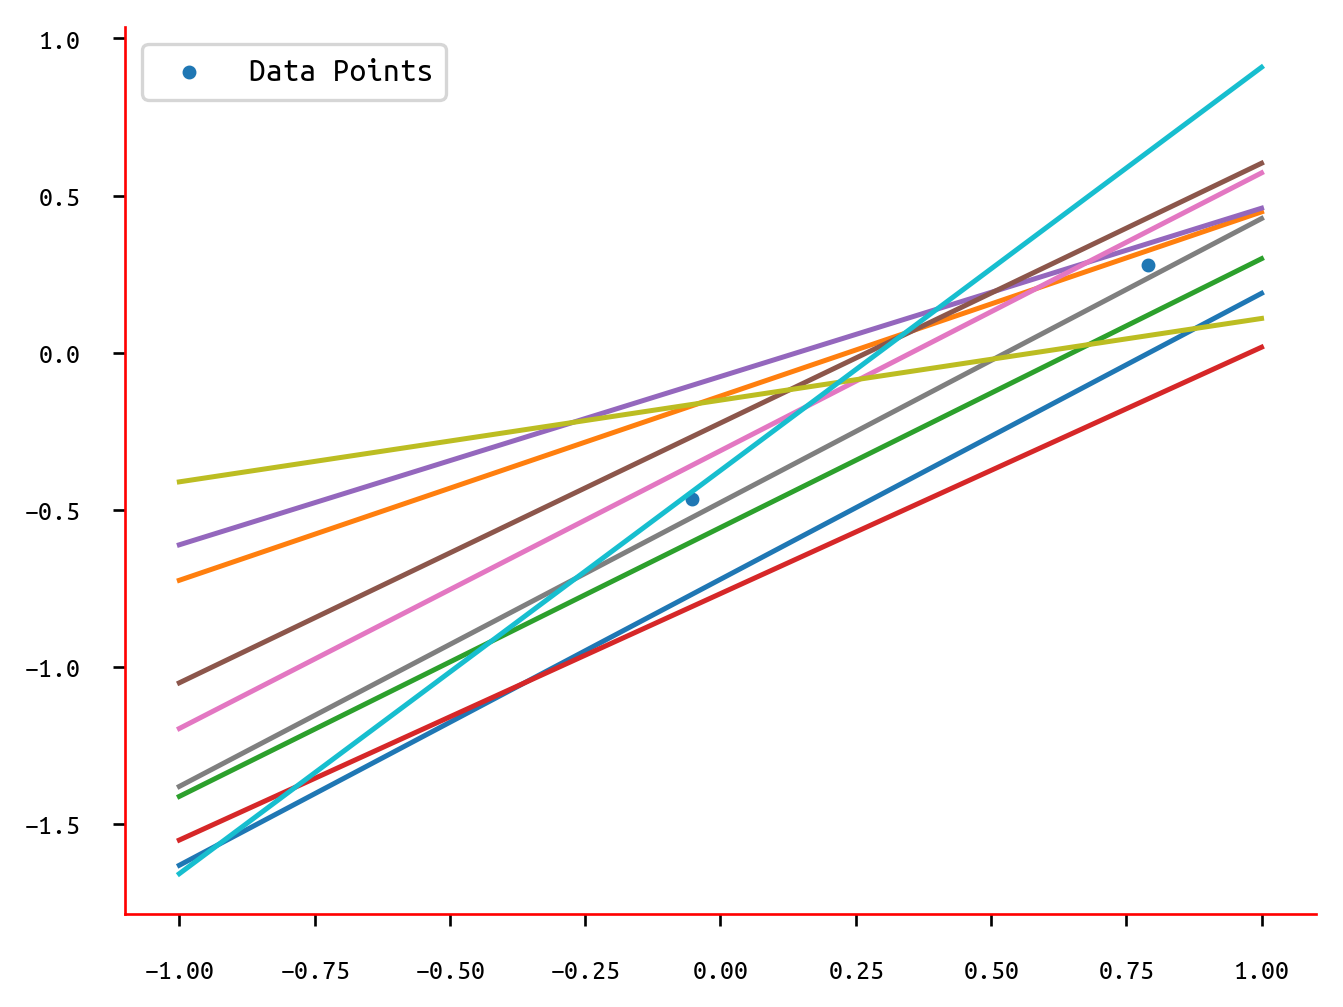
\includegraphics[height=275px]{includes/plots/q4c/predictive-models-2.png}
			\caption{Sampling of $w$ for N = $2$}
		\end{figure}

		\begin{figure}[h!]
			\centering
			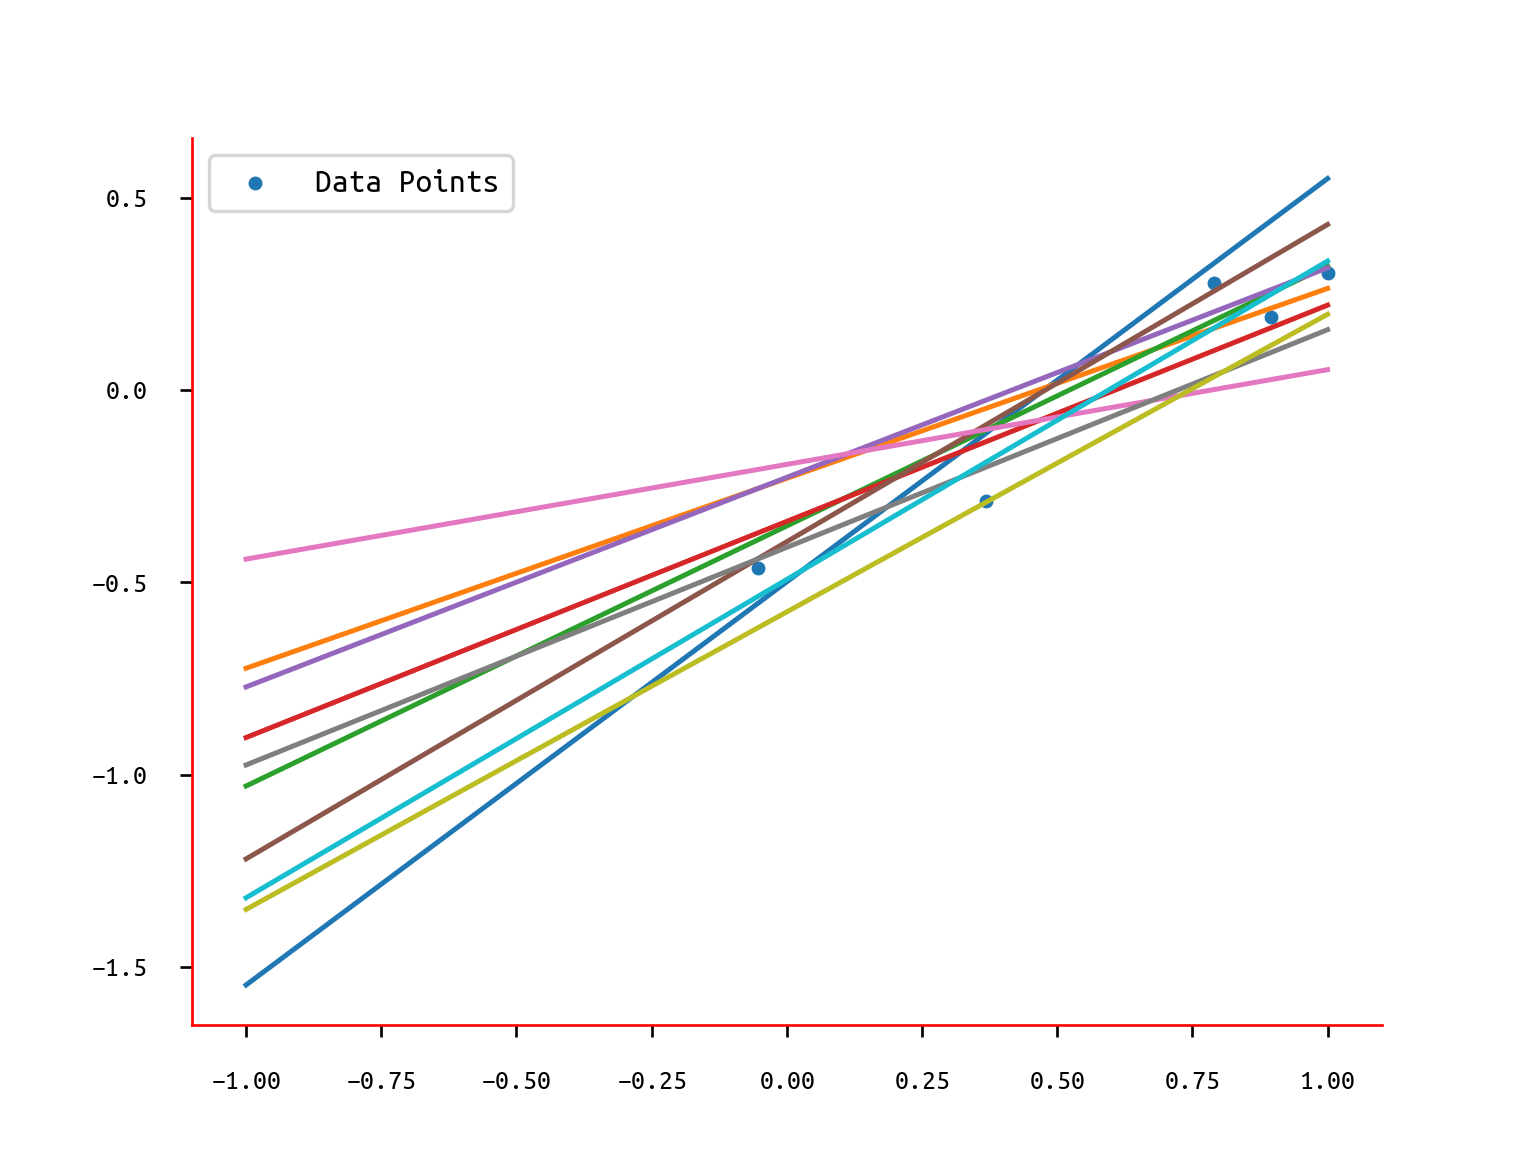
\includegraphics[height=275px]{includes/plots/q4c/predictive-models-3.png}
			\caption{Sampling of $w$ for N = $5$}
		\end{figure}

		\begin{figure}[h!]
			\centering
			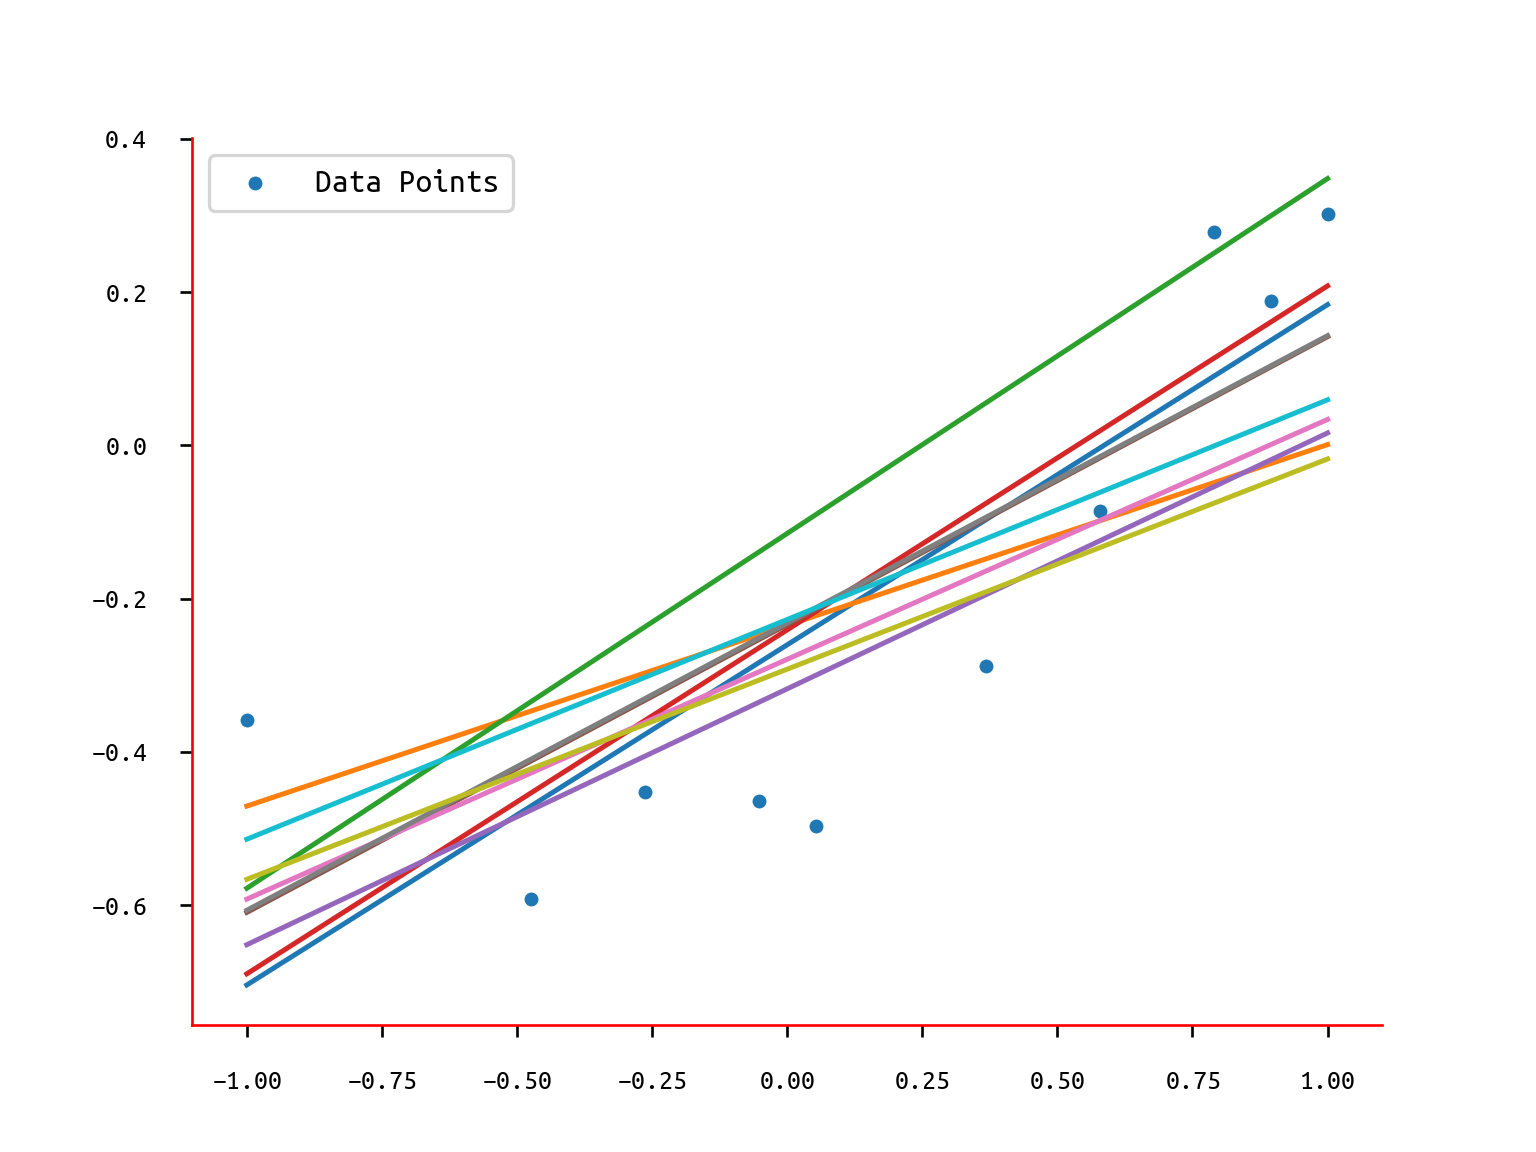
\includegraphics[height=275px]{includes/plots/q4c/predictive-models-4.png}
			\caption{Sampling of $w$ for N = $10$}
		\end{figure}

		\begin{figure}[h!]
			\centering
			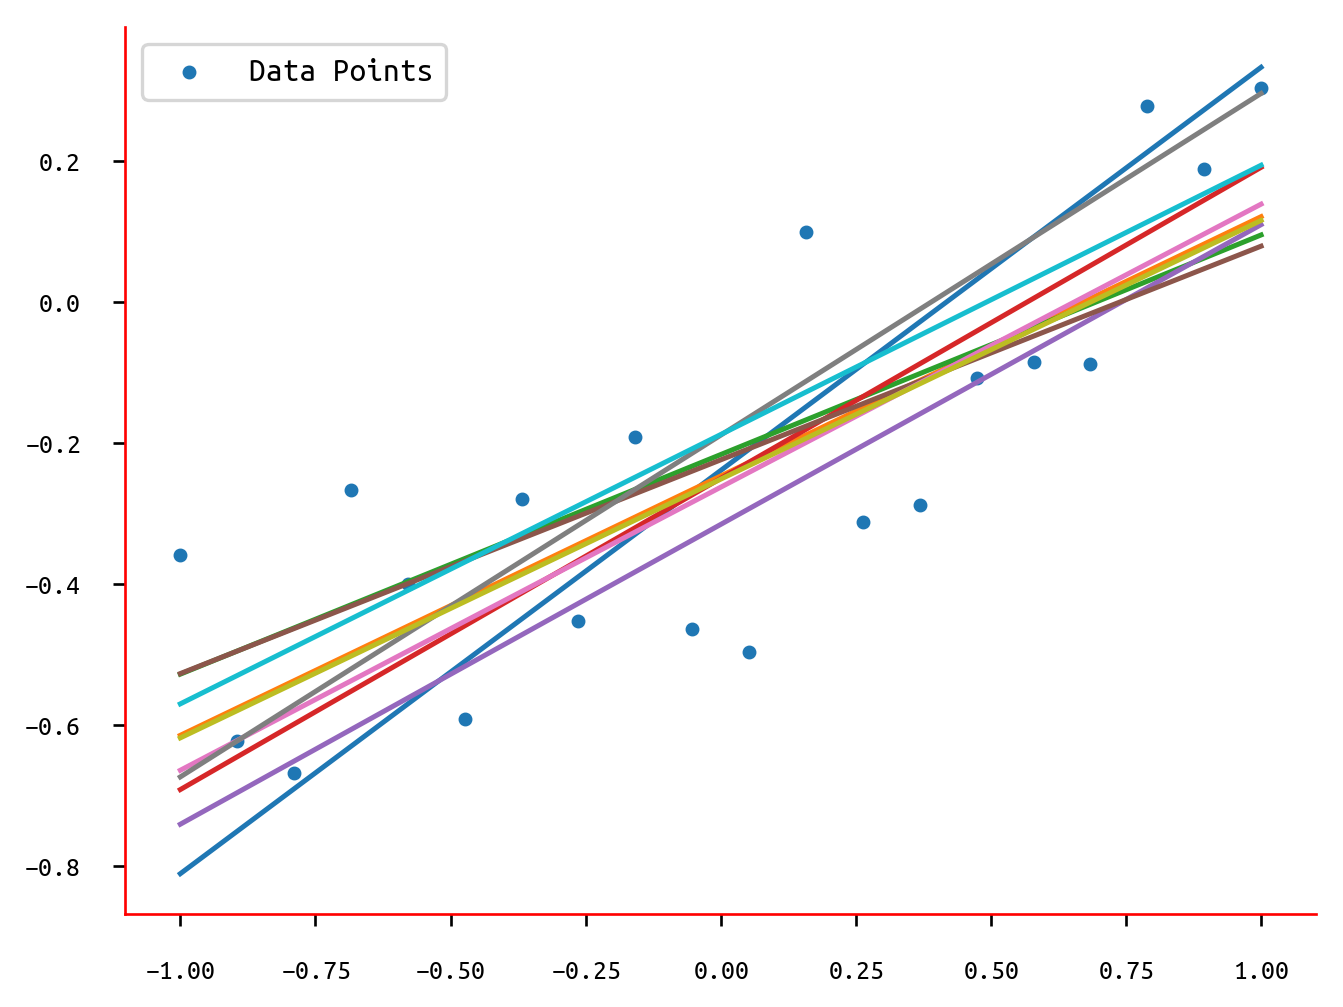
\includegraphics[height=275px]{includes/plots/q4c/predictive-models-5.png}
			\caption{Sampling of $w$ for N = $20$}
		\end{figure}

	\end{qsection}

	\clearpage

	\begin{qsection}{Observations}

		It can be very clearly seen from both the data in the first section, as well as from the figures that the absolute values of the covariance matrix are going down as the number of points are increasing.
		This is what is expected, as as the number of points increase, there is more surety about the fit (assuming the assumed model is a good fit, and there is no overfitting for small number of points), and therefore the variance in the inferred parameters will reduce.

		Another observation that can be made is that the mean of the posterior is converging, which makes sense from the computed value of the mean, that converges as the covariance matrix converges.

	\end{qsection}

\end{question}

\begin{question}

	Edward is a Turing-complete probabilistic programming language, integrated into TensorFlow (in python), providing significant speedups over existing probabilistic systems.

	Edward is built around an iterative process for probabilistic modeling.
	The process is as follows: formulating a model; inferring the model’s hidden structure; criticize how well the model captures the data’s generative process.
	As the tool criticizes the model’s fit to the data, it revises components of the model and repeats to form an iterative loop.

	\begin{enumerate}
		\item For \et{modeling}, Edward provides a language of random variables to construct a broad class of models: directed graphical models, stochastic neural networks, and programs with stochastic control flow
		\item For \et{inference}, Edward provides algorithms such as stochastic and black box variational inference, Hamiltonian Monte Carlo, and Stochastic Gradient Langevin Dynamics.
		\item For model \et{criticism}, Edward provides methods from scoring rules and predictive checks
	\end{enumerate}

	\begin{qsection}{Models}

		In Edward, all the models are represented as composotional graphs using random variables.
		They are essentially class objects with inbuilt methods such as computing the log density or sampling from the random variable.

		Furthermore, each random variable $X$ is associated to a tensor (multi-dimensional array) $X^\ast$, which represents a single sample $X^\ast ∼ X$.
		This association embeds the random variable into a computational graph, where nodes represent operations on tensors and edges represent tensors communicated between them.

		This design facilitates developing probabilistic programs in a computational graph framework.
		This makes it easy to compose random variables with complex deterministic structure such as deep neural networks, a diverse set of math operations, and third party libraries that build on the same framework.
		The design also enables compositions of random variables to capture complex stochastic structure.

		Edward allows all distributions supported by Tensorflow \footnote{\url{https://www.tensorflow.org/versions/master/api_guides/python/contrib.distributions}}.
		Using compositional graphical implementation, Edward supports a wide set of applications, such as Graphical Models, Neural Networks as well as Bayesian Nonparametrics using Collapsed Infinite Space (Gaussian Processes and Poisson Processes) or Lazily Defined Infinite Space (Dirichlet Processes).

	\end{qsection}

	\begin{qsection}{Inference Tasks}

		Edward supports many different ways to perform inference for different sets of problems.
		Inference is an abstract class which takes two inputs: a collection of latent variables, with model variables bound to posterior variables; and a collection of observed variables, with model variables bound to data.
		I is also possible to fine control the inference process.

		Edward also supports passing Model Parameters to compute point-estimates, or even doing conditional inference, by binding random variables to other random variables in the data itself.
		Latent variables can also be defined in the model without any posterior inference, and will be implicitly marginalized out using a single sample.

		The various classes of inference are discussed below.
		\clearpage

		\begin{qsubsection}{Variational Inference}

			By specifying the model parameters and an approximation (distribution) class, Edward allows us to perform Variational Inference to approximate the posterior over latent variables.

			It is also possible to compute MAP Estimates over the posterior usign Point Mass Random Variables as the approximation class.

		\end{qsubsection}

		\begin{qsubsection}{Monte Carlo Inference}

			Monte Carlo approximation simply approximates the posterior with an emperical distribution over the samples generated by updating one sample at a time.
			It is also possible to leverage the gradients and the graph structure, weherever applicable.

		\end{qsubsection}

		\begin{qsubsection}{Exact Inference}

			For some conjugate classes, it is possible to integrate out the paramters, thus computing the exact posterior, for example, exponential class of distributions.
			This avoids the approximation of posterior and automatically derives exact expressions for classical Gibbs and mean-field updates.

		\end{qsubsection}

		\begin{qsubsection}{Hybrid Algorithms}

			Hybrid Algorithms use different class of inference for different variables in the model, for example the EM algorithm with E-step over local (latent) variables and M-step over global variables (model parameters).

		\end{qsubsection}

		\begin{qsubsection}{Message Passing Algorithms}

			Edward allows inference using Message Passing, which operates on the posterior distribution using a collection of local inferences.
			With TensorFlow's distributed training, compositionality enables distributed message passing over a cluster with many workers.

			This extends to many algorithms, such as classical message passing, Gibbs sampling, expectation propogation, etc.
			In all of these, Edward is built to perform local inferences split over infiviual random variables.

		\end{qsubsection}

	\end{qsection}

	\begin{qsection}{Data Subsampling}

		Edward supports inference steps after looking at only partial data (sample).
		Only certain algorithms, such as MAP Estimation, KL Divergence and Stochastic Gradient Langevin Dynamics, support data subsampling.

	\end{qsection}

	\begin{qsection}{Model Criticism}

		Model Criticism helps justify the model as an approximation of the true data distribution.
		Edward explores model criticism using point-based evaluations, such as mean squared error, or posterior predictive checks, for making probabilistic assessments of the model fit using discrepancy functions.

	\end{qsection}

\end{question}

\begin{thebibliography}{10}
	\bibitem{matrix-cookbook}
		Matrix Cookbook.
		\quad
		\et{Kaare Brandt Petersen, Michael Syskind Pedersen} \\
		\href{http://www.matrixcookbook.com}{\url{http://www.matrixcookbook.com}}

	\bibitem{prml}
		Pattern Recongnition and Machine Learning.
		\; 2006.
		\quad
		\et{Christopher M.
		Bishop}

	\bibitem{wiki-order-of-integration}
		Order of Integration (n.d.)
		\et{Wikipedia} \\
		\href{https://en.wikipedia.org/wiki/Order_of_integration_(calculus)}{\url{https://en.wikipedia.org/wiki/Order_of_integration_(calculus)}}

	\bibitem{wiki-mgf}
		Moment Generating Function
		\et{Wikipedia} \\
		\href{https://en.wikipedia.org/wiki/Moment-generating_function}{\url{https://en.wikipedia.org/wiki/Moment-generating_function}}
\end{thebibliography}

\end{document}
